% Copyright (C) 2009 Romain Goffe, Alexandre Dupas
% Copyright (C) 2008 Kevin W. Hamlen
%
% This program is free software; you can redistribute it and/or
% modify it under the terms of the GNU General Public License
% as published by the Free Software Foundation; either version 2
% of the License, or (at your option) any later version.
%
% This program is distributed in the hope that it will be useful,
% but WITHOUT ANY WARRANTY; without even the implied warranty of
% MERCHANTABILITY or FITNESS FOR A PARTICULAR PURPOSE.  See the
% GNU General Public License for more details.
%
% You should have received a copy of the GNU General Public License
% along with this program; if not, write to the Free Software
% Foundation, Inc., 51 Franklin Street, Fifth Floor, Boston,
% MA  02110-1301, USA.
%
% The latest version of this program can be obtained from
% http://songs.sourceforge.net.
%
% Modified to serve personnal purposes. Newer versions can be 
% obtained from http://www.lohrun.net.

\documentclass[chorded]{crepbook}
\usepackage[utf8]{inputenc}
\usepackage[pdftex]{graphicx, color}
\usepackage[english,french]{babel}

\newindex{titleidx}{volume1cbtitle}
\newauthorindex{authidx}{volume1cbauth}

\graphicspath{
  {img/},
}

\title{Recueil de chansons pour guitare}
\author{Romain Goffe \and Alexandre Dupas}
\subtitle{Tome 1}
\version{3.1}
\mail{crep@team-on-fire.com}

\picture{feel-the-music}
\picturecopyright{©foxygamergirl @ deviantart.com}

\footer{
  \begin{flushleft}
    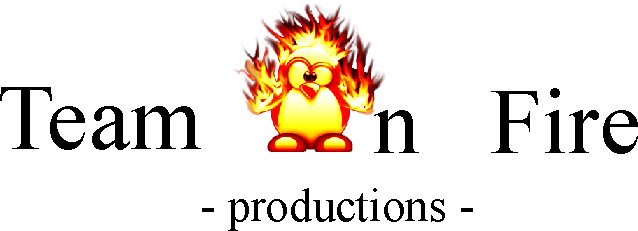
\includegraphics[width=3cm]{on-fire}
  \end{flushleft}
}

\licence{%License Creative Commons
\begin{center} \textbf{\LARGE{Creative Commons\footnote{Creative Commons peut être contacté a \url{http://creativecommons.org/}.} Legal Code}} \end{center}

\vspace{2cm}

Vous êtes libres:

\vspace{0.5cm}
\begin{itemize}
\item de reproduire, distribuer et communiquer cette création au public
\item de modifier cette création
\end{itemize}
\vspace{1cm}

Selon les conditions suivantes:

\vspace{0.5cm}
\begin{itemize}
\item \textbf{Paternité}. Vous devez citer le nom de l’auteur original
  de la manière indiquée par l’auteur de l’oeuvre ou le titulaire des
  droits qui vous confère cette autorisation (mais pas d’une manière
  qui suggérerait qu’ils vous soutiennent ou approuvent votre
  utilisation de l’\oe{}uvre).
\item \textbf{Pas d’Utilisation Commerciale}. Vous n’avez pas le droit
  d’utiliser cette création à des fins commerciales.
\item \textbf{Partage des Conditions Initiales à l’Identique}. Si vous
  modifiez, transformez ou adaptez cette création, vous n’avez le
  droit de distribuer la création qui en résulte que sous un contrat
  identique a celui-ci.
\end{itemize}

\vspace{1cm}
\begin{center}
  \begin{tabular}{|l|}
    \hline - A chaque réutilisation ou distribution de cette création,
    vous devez faire\\ apparaître clairement au public les conditions
    contractuelles de sa mise à\\ disposition.\\ - Chacune de ces
    conditions peut être levée si vous obtenez l’autorisation
    du\\ titulaire des droits sur cette \oe{}uvre.\\ - Rien dans ce
    contrat ne diminue ou ne restreint le droit moral de l’auteur
    ou\\ des auteurs.\\ \hline
  \end{tabular}
\end{center}

\vspace{1cm}

\begin{itemize}
\item Toutes les tablatures sont des représentations d'interprétations
  personnelles et approximatives de chansons protégées par droits
  d'auteurs. Conformément à l'article L.122-5 du Code de la propriété
  intellectuelle, l'utilisation de ces tablatures est strictement
  réservé à un usage personnel et pédagogique. Ce recueil de chansons
  n'a absolument aucune vocation commerciale et joue sur
  l'autorisation tacite des auteurs et des ayants droits, pensant que
  la publication de ces tablatures représente plutôt une publicité
  positive à leur égard. Cependant, si un auteur ou une société
  acréditée pense que ces tablatures sont utilisées d'une manière
  susceptible de porter atteinte à ses droits et désire s'opposer à la
  publication de ses tablatures, merci de nous contacter à
  \url{crep@team-on-fire.com} et celles-ci seront immédiatement
  retirées du site.
\item Les illustrations proviennent en majeur partie de la Tux factory
  du site: \url{http://www.crystalxp.net/}.
\item Ce document est écrit en LaTex, d'après le style du projet Songs
  disponible à l'adresse: \url{http://songs.sourceforge.net/}
\end{itemize}

\vspace{1cm}
\image{license}{2.5}
% Fin de la License
}

\begin{document}

\maketitle

\showindex{Index des chansons}{titleidx}
\showindex{Index des auteurs}{authidx}

% desactivate ':' as an active character from babel[french]
\shorthandoff{:} 

\songsection{Chansons}
\begin{songs}{titleidx,authidx}
  % Copyright (C) 2009 Romain Goffe, Alexandre Dupas
% Copyright (C) 2008 Kevin W. Hamlen
%
% This program is free software; you can redistribute it and/or
% modify it under the terms of the GNU General Public License
% as published by the Free Software Foundation; either version 2
% of the License, or (at your option) any later version.
%
% This program is distributed in the hope that it will be useful,
% but WITHOUT ANY WARRANTY; without even the implied warranty of
% MERCHANTABILITY or FITNESS FOR A PARTICULAR PURPOSE.  See the
% GNU General Public License for more details.
%
% You should have received a copy of the GNU General Public License
% along with this program; if not, write to the Free Software
% Foundation, Inc., 51 Franklin Street, Fifth Floor, Boston,
% MA  02110-1301, USA.
%
% The latest version of this program can be obtained from
% http://songs.sourceforge.net.
%
% Modified to serve personnal purposes. Newer versions can be 
% obtained from http://www.lohrun.net.

\documentclass{crepbook}
\usepackage[bookmarks,bookmarksopen]{hyperref}
\usepackage[chorded]{songs}
\usepackage[utf8]{inputenc}
\usepackage[pdftex]{graphicx, color}
\usepackage[english,french]{babel}
\usepackage{fancybox}

\usepackage{songbook}

\newindex{titleidx}{volume1cbtitle}
\newauthorindex{authidx}{volume1cbauth}

\graphicspath{
  {img/},
}

\title{Recueil de chansons pour guitare}
\author{Romain Goffe \and Alexandre Dupas}
\subtitle{Tome 1}
\version{3.1}
\mail{crep@team-on-fire.com}

\picture{feel-the-music}
\picturecopyright{©foxygamergirl @ deviantart.com}

\footer{
  \begin{flushleft}
    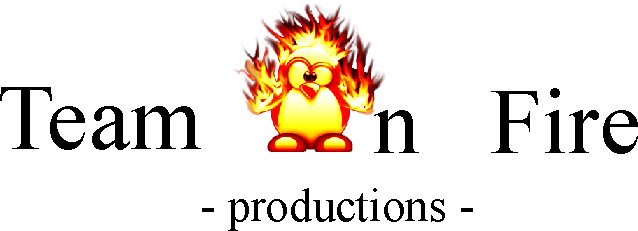
\includegraphics[width=3cm]{on-fire}
  \end{flushleft}
}

\licence{%License Creative Commons
\begin{center} \textbf{\LARGE{Creative Commons\footnote{Creative Commons peut être contacté a \url{http://creativecommons.org/}.} Legal Code}} \end{center}

\vspace{2cm}

Vous êtes libres:

\vspace{0.5cm}
\begin{itemize}
\item de reproduire, distribuer et communiquer cette création au public
\item de modifier cette création
\end{itemize}
\vspace{1cm}

Selon les conditions suivantes:

\vspace{0.5cm}
\begin{itemize}
\item \textbf{Paternité}. Vous devez citer le nom de l’auteur original
  de la manière indiquée par l’auteur de l’oeuvre ou le titulaire des
  droits qui vous confère cette autorisation (mais pas d’une manière
  qui suggérerait qu’ils vous soutiennent ou approuvent votre
  utilisation de l’\oe{}uvre).
\item \textbf{Pas d’Utilisation Commerciale}. Vous n’avez pas le droit
  d’utiliser cette création à des fins commerciales.
\item \textbf{Partage des Conditions Initiales à l’Identique}. Si vous
  modifiez, transformez ou adaptez cette création, vous n’avez le
  droit de distribuer la création qui en résulte que sous un contrat
  identique a celui-ci.
\end{itemize}

\vspace{1cm}
\begin{center}
  \begin{tabular}{|l|}
    \hline - A chaque réutilisation ou distribution de cette création,
    vous devez faire\\ apparaître clairement au public les conditions
    contractuelles de sa mise à\\ disposition.\\ - Chacune de ces
    conditions peut être levée si vous obtenez l’autorisation
    du\\ titulaire des droits sur cette \oe{}uvre.\\ - Rien dans ce
    contrat ne diminue ou ne restreint le droit moral de l’auteur
    ou\\ des auteurs.\\ \hline
  \end{tabular}
\end{center}

\vspace{1cm}

\begin{itemize}
\item Toutes les tablatures sont des représentations d'interprétations
  personnelles et approximatives de chansons protégées par droits
  d'auteurs. Conformément à l'article L.122-5 du Code de la propriété
  intellectuelle, l'utilisation de ces tablatures est strictement
  réservé à un usage personnel et pédagogique. Ce recueil de chansons
  n'a absolument aucune vocation commerciale et joue sur
  l'autorisation tacite des auteurs et des ayants droits, pensant que
  la publication de ces tablatures représente plutôt une publicité
  positive à leur égard. Cependant, si un auteur ou une société
  acréditée pense que ces tablatures sont utilisées d'une manière
  susceptible de porter atteinte à ses droits et désire s'opposer à la
  publication de ses tablatures, merci de nous contacter à
  \url{crep@team-on-fire.com} et celles-ci seront immédiatement
  retirées du site.
\item Les illustrations proviennent en majeur partie de la Tux factory
  du site: \url{http://www.crystalxp.net/}.
\item Ce document est écrit en LaTex, d'après le style du projet Songs
  disponible à l'adresse: \url{http://songs.sourceforge.net/}
\end{itemize}

\vspace{1cm}
\image{license}{2.5}
% Fin de la License
}

\begin{document}

\maketitle

\showindex{Index des chansons}{titleidx}
\showindex{Index des auteurs}{authidx}

% desactivate ':' as an active character from babel[french]
\shorthandoff{:} 

\songsection{Chansons}
\begin{songs}{titleidx,authidx}
  % Copyright (C) 2009 Romain Goffe, Alexandre Dupas
% Copyright (C) 2008 Kevin W. Hamlen
%
% This program is free software; you can redistribute it and/or
% modify it under the terms of the GNU General Public License
% as published by the Free Software Foundation; either version 2
% of the License, or (at your option) any later version.
%
% This program is distributed in the hope that it will be useful,
% but WITHOUT ANY WARRANTY; without even the implied warranty of
% MERCHANTABILITY or FITNESS FOR A PARTICULAR PURPOSE.  See the
% GNU General Public License for more details.
%
% You should have received a copy of the GNU General Public License
% along with this program; if not, write to the Free Software
% Foundation, Inc., 51 Franklin Street, Fifth Floor, Boston,
% MA  02110-1301, USA.
%
% The latest version of this program can be obtained from
% http://songs.sourceforge.net.
%
% Modified to serve personnal purposes. Newer versions can be 
% obtained from http://www.lohrun.net.

\documentclass{crepbook}
\usepackage[bookmarks,bookmarksopen]{hyperref}
\usepackage[chorded]{songs}
\usepackage[utf8]{inputenc}
\usepackage[pdftex]{graphicx, color}
\usepackage[english,french]{babel}
\usepackage{fancybox}

\usepackage{songbook}

\newindex{titleidx}{volume1cbtitle}
\newauthorindex{authidx}{volume1cbauth}

\graphicspath{
  {img/},
}

\title{Recueil de chansons pour guitare}
\author{Romain Goffe \and Alexandre Dupas}
\subtitle{Tome 1}
\version{3.1}
\mail{crep@team-on-fire.com}

\picture{feel-the-music}
\picturecopyright{©foxygamergirl @ deviantart.com}

\footer{
  \begin{flushleft}
    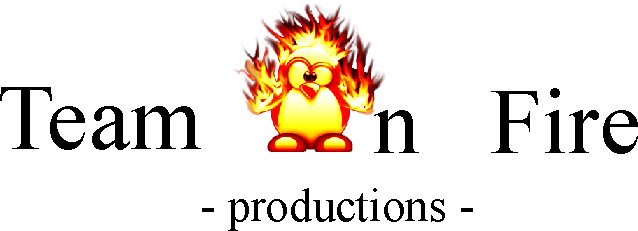
\includegraphics[width=3cm]{on-fire}
  \end{flushleft}
}

\licence{%License Creative Commons
\begin{center} \textbf{\LARGE{Creative Commons\footnote{Creative Commons peut être contacté a \url{http://creativecommons.org/}.} Legal Code}} \end{center}

\vspace{2cm}

Vous êtes libres:

\vspace{0.5cm}
\begin{itemize}
\item de reproduire, distribuer et communiquer cette création au public
\item de modifier cette création
\end{itemize}
\vspace{1cm}

Selon les conditions suivantes:

\vspace{0.5cm}
\begin{itemize}
\item \textbf{Paternité}. Vous devez citer le nom de l’auteur original
  de la manière indiquée par l’auteur de l’oeuvre ou le titulaire des
  droits qui vous confère cette autorisation (mais pas d’une manière
  qui suggérerait qu’ils vous soutiennent ou approuvent votre
  utilisation de l’\oe{}uvre).
\item \textbf{Pas d’Utilisation Commerciale}. Vous n’avez pas le droit
  d’utiliser cette création à des fins commerciales.
\item \textbf{Partage des Conditions Initiales à l’Identique}. Si vous
  modifiez, transformez ou adaptez cette création, vous n’avez le
  droit de distribuer la création qui en résulte que sous un contrat
  identique a celui-ci.
\end{itemize}

\vspace{1cm}
\begin{center}
  \begin{tabular}{|l|}
    \hline - A chaque réutilisation ou distribution de cette création,
    vous devez faire\\ apparaître clairement au public les conditions
    contractuelles de sa mise à\\ disposition.\\ - Chacune de ces
    conditions peut être levée si vous obtenez l’autorisation
    du\\ titulaire des droits sur cette \oe{}uvre.\\ - Rien dans ce
    contrat ne diminue ou ne restreint le droit moral de l’auteur
    ou\\ des auteurs.\\ \hline
  \end{tabular}
\end{center}

\vspace{1cm}

\begin{itemize}
\item Toutes les tablatures sont des représentations d'interprétations
  personnelles et approximatives de chansons protégées par droits
  d'auteurs. Conformément à l'article L.122-5 du Code de la propriété
  intellectuelle, l'utilisation de ces tablatures est strictement
  réservé à un usage personnel et pédagogique. Ce recueil de chansons
  n'a absolument aucune vocation commerciale et joue sur
  l'autorisation tacite des auteurs et des ayants droits, pensant que
  la publication de ces tablatures représente plutôt une publicité
  positive à leur égard. Cependant, si un auteur ou une société
  acréditée pense que ces tablatures sont utilisées d'une manière
  susceptible de porter atteinte à ses droits et désire s'opposer à la
  publication de ses tablatures, merci de nous contacter à
  \url{crep@team-on-fire.com} et celles-ci seront immédiatement
  retirées du site.
\item Les illustrations proviennent en majeur partie de la Tux factory
  du site: \url{http://www.crystalxp.net/}.
\item Ce document est écrit en LaTex, d'après le style du projet Songs
  disponible à l'adresse: \url{http://songs.sourceforge.net/}
\end{itemize}

\vspace{1cm}
\image{license}{2.5}
% Fin de la License
}

\begin{document}

\maketitle

\showindex{Index des chansons}{titleidx}
\showindex{Index des auteurs}{authidx}

% desactivate ':' as an active character from babel[french]
\shorthandoff{:} 

\songsection{Chansons}
\begin{songs}{titleidx,authidx}
  % Copyright (C) 2009 Romain Goffe, Alexandre Dupas
% Copyright (C) 2008 Kevin W. Hamlen
%
% This program is free software; you can redistribute it and/or
% modify it under the terms of the GNU General Public License
% as published by the Free Software Foundation; either version 2
% of the License, or (at your option) any later version.
%
% This program is distributed in the hope that it will be useful,
% but WITHOUT ANY WARRANTY; without even the implied warranty of
% MERCHANTABILITY or FITNESS FOR A PARTICULAR PURPOSE.  See the
% GNU General Public License for more details.
%
% You should have received a copy of the GNU General Public License
% along with this program; if not, write to the Free Software
% Foundation, Inc., 51 Franklin Street, Fifth Floor, Boston,
% MA  02110-1301, USA.
%
% The latest version of this program can be obtained from
% http://songs.sourceforge.net.
%
% Modified to serve personnal purposes. Newer versions can be 
% obtained from http://www.lohrun.net.

\documentclass{crepbook}
\usepackage[bookmarks,bookmarksopen]{hyperref}
\usepackage[chorded]{songs}
\usepackage[utf8]{inputenc}
\usepackage[pdftex]{graphicx, color}
\usepackage[english,french]{babel}
\usepackage{fancybox}

\usepackage{songbook}

\newindex{titleidx}{volume1cbtitle}
\newauthorindex{authidx}{volume1cbauth}

\graphicspath{
  {img/},
}

\title{Recueil de chansons pour guitare}
\author{Romain Goffe \and Alexandre Dupas}
\subtitle{Tome 1}
\version{3.1}
\mail{crep@team-on-fire.com}

\picture{feel-the-music}
\picturecopyright{©foxygamergirl @ deviantart.com}

\footer{
  \begin{flushleft}
    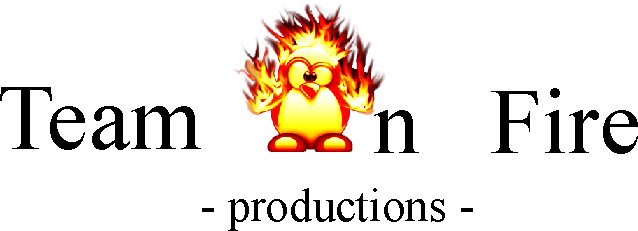
\includegraphics[width=3cm]{on-fire}
  \end{flushleft}
}

\licence{\input{license.tex}}

\begin{document}

\maketitle

\showindex{Index des chansons}{titleidx}
\showindex{Index des auteurs}{authidx}

% desactivate ':' as an active character from babel[french]
\shorthandoff{:} 

\songsection{Chansons}
\begin{songs}{titleidx,authidx}
  \input{volume-1.sbd}
\end{songs}

\end{document}

\end{songs}

\end{document}

\end{songs}

\end{document}

\end{songs}

\end{document}
